\section{Resultaten}
De
Hallo
[1-D model]
\begin{figure}[H]
    \centering
    \subfloat[]{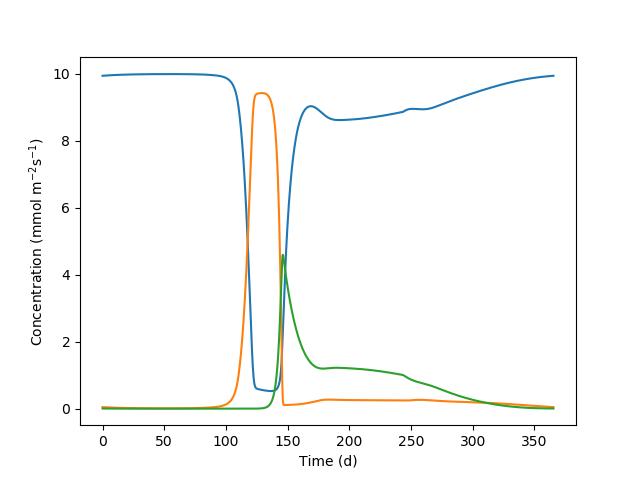
\includegraphics[width=0.5\textwidth]{figures/simple.png}}
    \subfloat[]{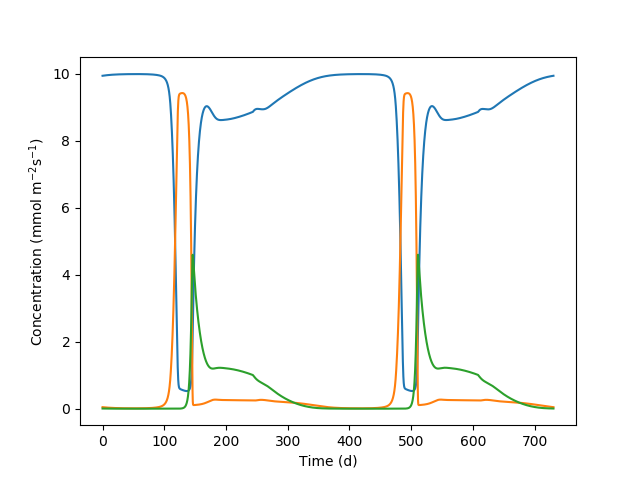
\includegraphics[width=0.5\textwidth, height=0.35\textwidth]{figures/simple_long.png}}

    \caption{Het één dimensionale model. De Nutrienten concentratie (blauw), plankton concentratie (orange) en de herbivoren concentratie (groen) weergegeven tegen de tijd. (a) tijd schaal van één jaar. (b) tijd schaal van twee jaar.
    }
    \label{fig:Res:Simple}
\end{figure}
In figuur \ref{fig:Res:Simple} is de jaarlijkse plankton bloei te zien die begint rond de 100ste dag na midwinter. Dit correspondeert aan eind maart of de begin van de lente. Na 30 dagen neemt de plankton concentratie weer af tot iets onder de gemiddelde waardes. Na de plankton piek is er te zien dat er een herbivoren concentratie piek is. De herbivoren concentratie blijft tot de 200ste dag relatief stabiel tot dat deze uiteindelijk ook afneemt.\\
\\
Om de ruimtelijke invloed te meten moet er gekozen worden voor een in ruimte varierende begin conditie. In dit onderzoek is er gekozen voor een gaussische begin conditie zoals zichtbaar in figuur \ref{fig:Res:IC}. Deze zou over een kunnen komen met een stikstof dumpend schip dat onlangs voorbij is gevaren.

\begin{figure}[H]
    \centering
    {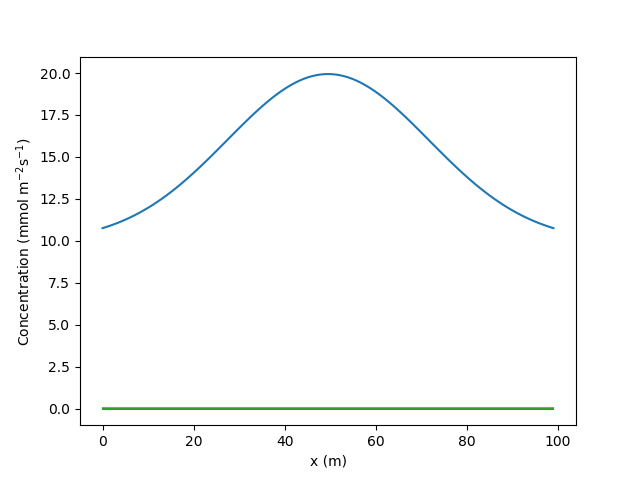
\includegraphics[width=0.5\textwidth]{figures/Inital_Condition.png}}
    \caption{ De begin conditie van het model met de Nutrienten concentratie (blauw), plankton concentratie (orange) en de herbivoren concentratie (groen). Hierin is te zien dat de stikstof concentratie een gausische curve beschrijft in de ruimte. Ook is te zien dat de begin waardes van de herbivoren en plankton concentratie plaats onafhankelijk zijn.
    }
    \label{fig:Res:IC}
\end{figure}

Om de effecten van de stroming en diffusie apart te kunnen analyseren zijn in figuur \ref{fig:Res:Color0} alle andere effecten uitgezet. 
\begin{figure}[H]
    \centering
    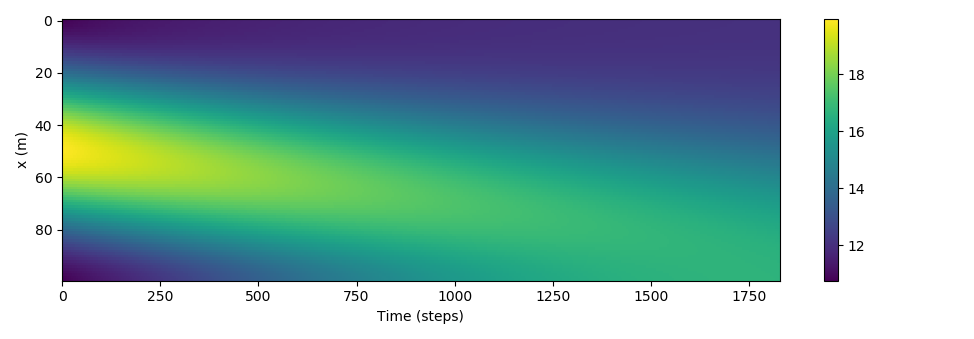
\includegraphics[width=0.8\textwidth]{figures/color_plot_0Flow.png}
   \hfill
    \caption{De invloed van enkel de stroming en diffusie op de begin conditie. Hierin is ruimte tegen de tijd weergegeven met de hierin de concentratie als kleur. Welke waarde met welke concentratie correspondeert is te zien in de bij staande legenda.}
    \label{fig:Res:Color0}
\end{figure}

In figuur \ref{fig:Res:Color0} is zichtbaar dat de gausisch beginwaarde van figuur \ref{fig:Res:IC} in breedte toeneemt terwijl de piek in hoogte afneemt en naar beneden verschuift door middel van de stroming.

\begin{figure}[H]
   \centering
   \subfloat[]{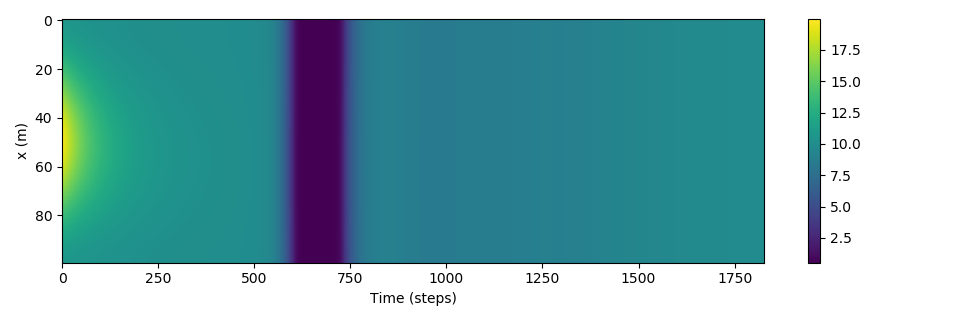
\includegraphics[width=0.5\textwidth]{figures/color_plot_1N.png}}
   \hfill
   \subfloat[]{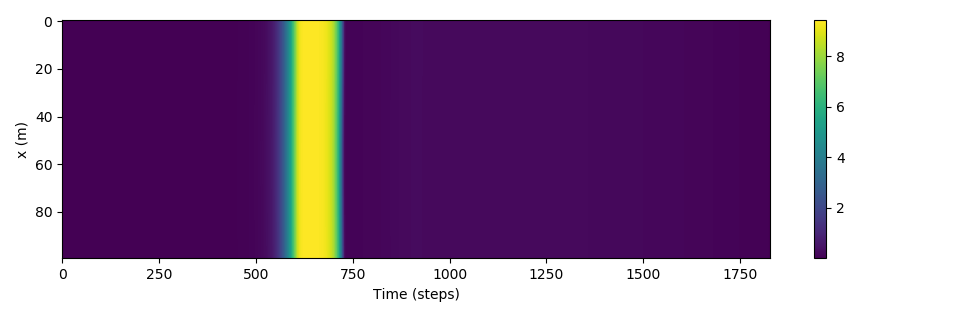
\includegraphics[width=0.5\textwidth]{figures/color_plot_1P.png}}
   \hfill   
   \subfloat[]{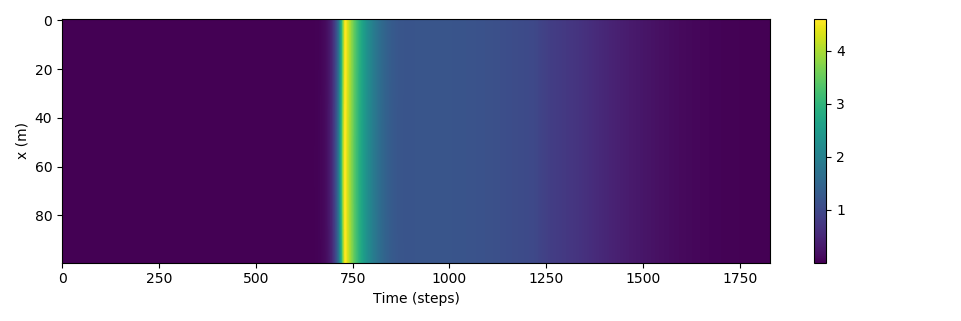
\includegraphics[width=0.5\textwidth]{figures/color_plot_1H.png}}
   \hfill
    \caption{}
    \label{fig:Res:Color1}
\end{figure}

\begin{figure}[H]
    \centering
   \subfloat[]{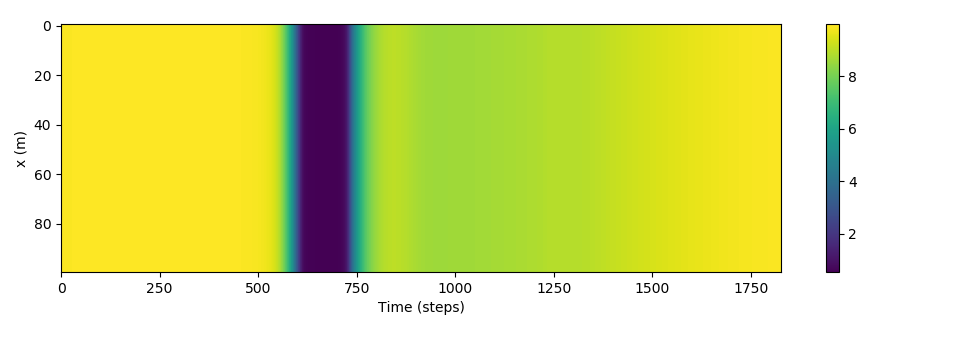
\includegraphics[width=0.5\textwidth]{figures/color_plot_1N2.png}}
   \hfill
   \subfloat[]{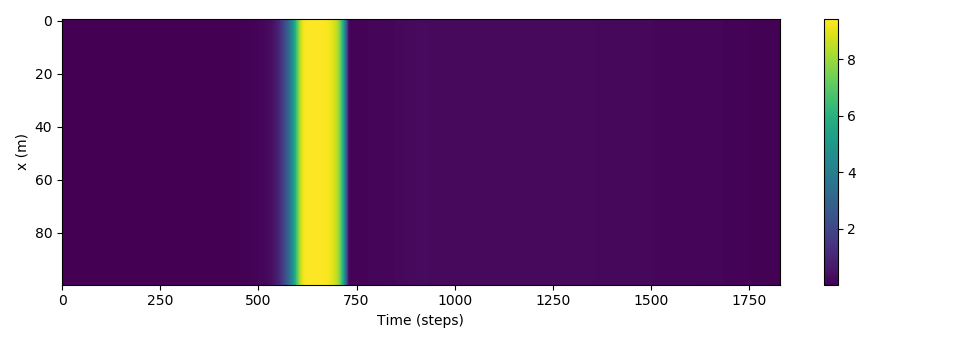
\includegraphics[width=0.5\textwidth]{figures/color_plot_1P2.png}}
   \hfill
   \subfloat[]{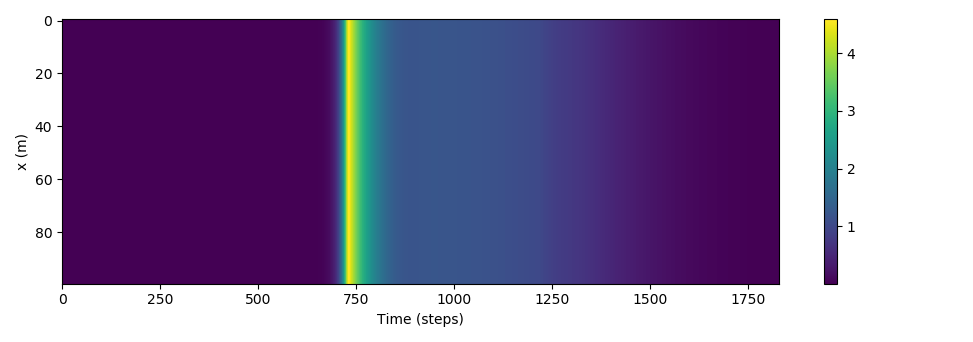
\includegraphics[width=0.5\textwidth]{figures/color_plot_1H2.png}}
   \hfill
   \caption{Caption}
   \label{fig:Res:Color2}
\end{figure}

\begin{figure}[H]
\centering
   \hfill
   \subfloat[]{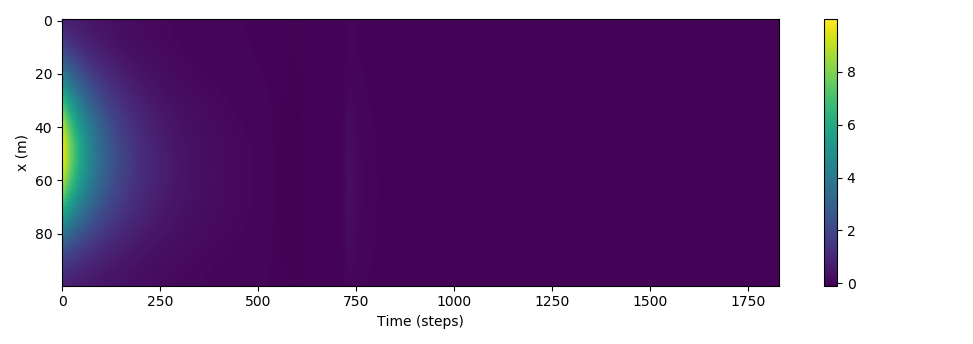
\includegraphics[width=\0.5\textwidth]{figures/color_plot_1N3.png}}
   \hfill
   \subfloat[]{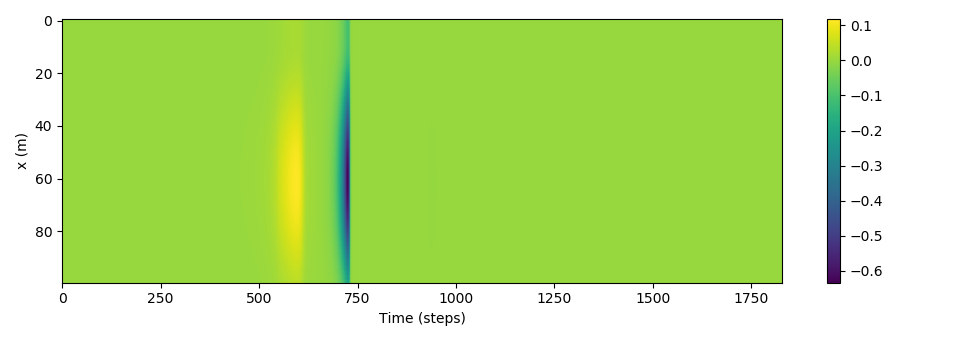
\includegraphics[width=0.5\textwidth]{figures/color_plot_1P3.png}}
   \hfill
   \subfloat[]{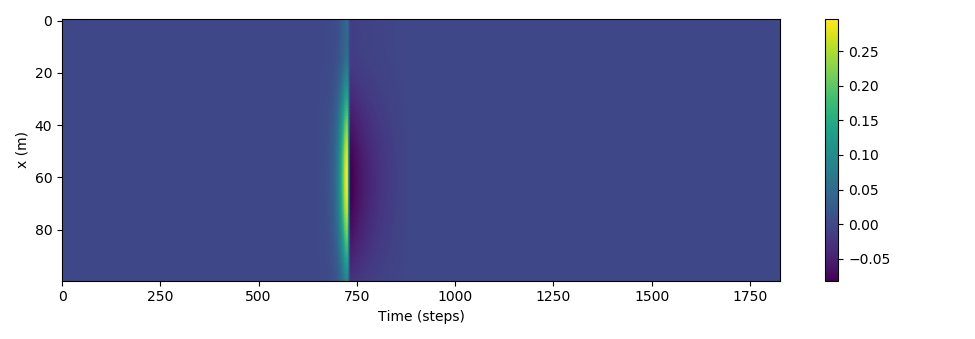
\includegraphics[width=0.5\textwidth]{figures/color_plot_1H3.png}}
   \hfill
   \caption{Caption}
    \label{fig:Res:Color3}
\end{figure}